\documentclass[reqno,a4paper,11pt]{amsart}
\usepackage[utf8]{inputenc}
\usepackage{amsmath, amssymb, amsthm, mathtools,times,comment}
\usepackage[T1]{fontenc}
\usepackage{xcolor}
\usepackage{tikz}
\usetikzlibrary{3d}
\usetikzlibrary{calc}
\usetikzlibrary{shapes.geometric}

\begin{document}

    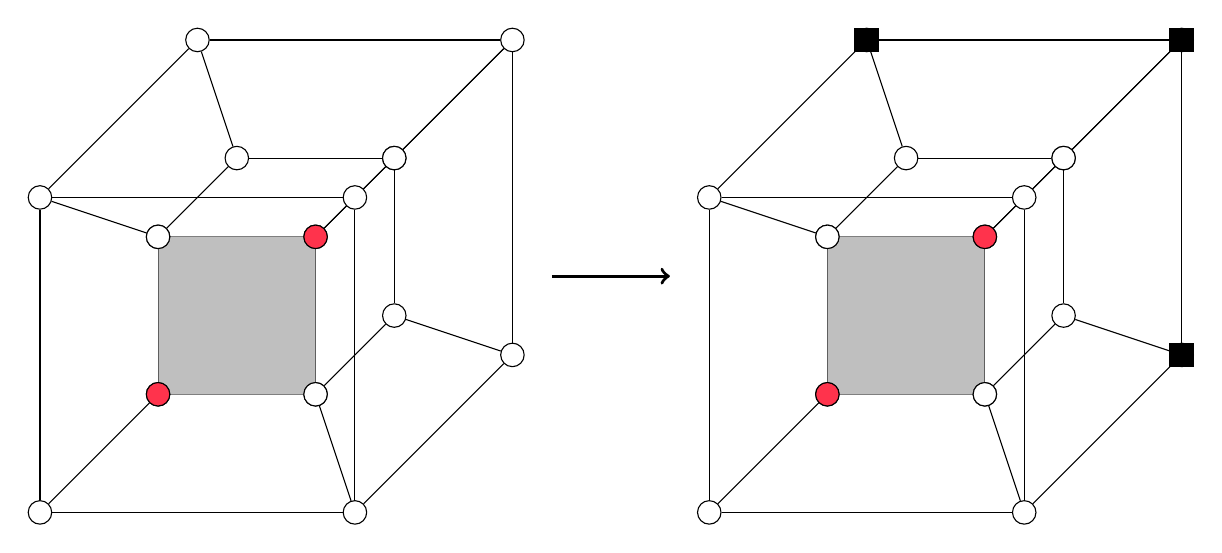
\begin{tikzpicture}
\definecolor{myred}{rgb}{1,0.2,0.3}
\definecolor{mycand}{rgb}{1,1,0}
\tikzstyle{vertex}= [circle,draw, fill = white, inner sep=3pt]
\tikzstyle{infvertex} = [circle,draw, fill = myred, inner sep=3pt]
\tikzstyle{candvertex} = [regular polygon, regular polygon sides=4,draw, fill = black, inner sep=3pt]
\def\lengths{2};
\def\lengthl{4}
\coordinate (anchor1) at (1.5,1.5);
\coordinate (anchor2) at (0,0);
\coordinate (anchor3) at (10,1.5);
\coordinate (anchor4) at ($(anchor3) +(anchor2)-(anchor1) $);


\node[vertex] (v1) at (anchor1) {};

\node[vertex] (v2) at ($(anchor1) +(\lengths,0)$){};
\node[vertex] (v3) at ($(anchor1) +(0,\lengths)$){};
\node[vertex] (v4) at ($(anchor1) +(\lengths,\lengths)$){};

\node[vertex] (v5) at ($(anchor1) +(\lengths,0)+(0.5*\lengths,0.5*\lengths)$){};
\node[vertex] (v6) at ($(anchor1) +(0,\lengths)+(0.5*\lengths,0.5*\lengths)$){};
\node[vertex] (v7) at ($(anchor1) +(\lengths,\lengths)+(0.5*\lengths,0.5*\lengths)$){};

\filldraw[fill = gray,opacity = 0.5] (v1.center)--(v2.center)--(v4.center)--(v3.center)--cycle;
\node[vertex] at (v2) {};
\node[vertex] at (v3) {};
\node[infvertex] at(v1) {};
\node[infvertex] at(v4) {};
\draw[-] (v5)--(v7)--(v6);
\draw[-] (v2)--(v5);
\draw[-] (v3)--(v6);
\draw[-] (v4)--(v7);


\node[vertex] (w1) at (anchor2) {};

\node[vertex] (w2) at ($(anchor2) +(\lengthl,0)$){};
\node[vertex] (w3) at ($(anchor2) +(0,\lengthl)$){};
\node[vertex] (w4) at ($(anchor2) +(\lengthl,\lengthl)$){};

\node[vertex] (w5) at ($(anchor2) +(\lengthl,0)+(0.5*\lengthl,0.5*\lengthl)$){};
\node[vertex] (w6) at ($(anchor2) +(0,\lengthl)+(0.5*\lengthl,0.5*\lengthl)$){};
\node[vertex] (w7) at ($(anchor2) +(\lengthl,\lengthl)+(0.5*\lengthl,0.5*\lengthl)$){};

\draw[-] (w1)--(w2)--(w4)--(w3)--(w1);
\draw[-] (w5)--(w7)--(w6);
\draw[-] (w2)--(w5);
\draw[-] (w3)--(w6);
\draw[-] (w4)--(w7);
\node[vertex]  at (v7){};

\foreach \i in {1,...,7}
\draw[-] (v\i) --(w\i);


\coordinate (anchor1) at (anchor3);
\coordinate (anchor2) at (anchor4);


\node[vertex] (v1) at (anchor1) {};

\node[vertex] (v2) at ($(anchor1) +(\lengths,0)$){};
\node[vertex] (v3) at ($(anchor1) +(0,\lengths)$){};
\node[vertex] (v4) at ($(anchor1) +(\lengths,\lengths)$){};

\node[vertex] (v5) at ($(anchor1) +(\lengths,0)+(0.5*\lengths,0.5*\lengths)$){};
\node[vertex] (v6) at ($(anchor1) +(0,\lengths)+(0.5*\lengths,0.5*\lengths)$){};
\node[vertex] (v7) at ($(anchor1) +(\lengths,\lengths)+(0.5*\lengths,0.5*\lengths)$){};

\filldraw[fill = gray,opacity = 0.5] (v1.center)--(v2.center)--(v4.center)--(v3.center)--cycle;
\node[vertex] at (v2) {};
\node[vertex] at (v3) {};
\node[infvertex] at(v1) {};
\node[infvertex] at(v4) {};
\draw[-] (v5)--(v7)--(v6);
\draw[-] (v2)--(v5);
\draw[-] (v3)--(v6);
\draw[-] (v4)--(v7);


\node[vertex] (w1) at (anchor2) {};

\node[vertex] (w2) at ($(anchor2) +(\lengthl,0)$){};
\node[vertex] (w3) at ($(anchor2) +(0,\lengthl)$){};
\node[vertex] (w4) at ($(anchor2) +(\lengthl,\lengthl)$){};

\node[vertex] (w5) at ($(anchor2) +(\lengthl,0)+(0.5*\lengthl,0.5*\lengthl)$){};
\node[vertex] (w6) at ($(anchor2) +(0,\lengthl)+(0.5*\lengthl,0.5*\lengthl)$){};
\node[vertex] (w7) at ($(anchor2) +(\lengthl,\lengthl)+(0.5*\lengthl,0.5*\lengthl)$){};

\draw[-] (w1)--(w2)--(w4)--(w3)--(w1);
\draw[-] (w5)--(w7)--(w6);
\draw[-] (w2)--(w5);
\draw[-] (w3)--(w6);
\draw[-] (w4)--(w7);
\node[vertex]  at (v7){};

\foreach \i in {1,...,7}
\draw[-] (v\i) --(w\i);

\node[candvertex] at (w5) {};
\node[candvertex] at (w6) {};
\node[candvertex] at (w7) {};
\draw[->, very thick] (6.5,3)--(8,3) ;

\end{tikzpicture}

\end{document}